\documentclass[a4paper, UTF8]{article}
\usepackage{graphicx}
\usepackage{subfigure}
\usepackage{amsmath}
\usepackage{makecell}
\usepackage[utf8]{inputenc}
\usepackage[space]{ctex} %中文包
\usepackage{listings} %放代码
\usepackage{xcolor} %代码着色宏包
\usepackage{CJK} %显示中文宏包
\usepackage{float}
\usepackage{makecell}
\usepackage{diagbox}
\usepackage{bm}
\usepackage{ulem} 
\usepackage{amssymb}
\usepackage{soul}
\usepackage{color}
\usepackage{geometry}
\usepackage{fancybox} %花里胡哨的盒子
\usepackage{xhfill} %填充包, 可画分割线 https://www.latexstudio.net/archives/8245
\usepackage{multicol} %多栏包
\usepackage{enumerate} %可以方便地自定义枚举标题
\usepackage{multirow} %表格中多行单元格合并
\usepackage{wasysym} %可以使用wasysym里的一堆奇奇怪怪的符号

\geometry{left = 1cm, right = 1cm, top=1cm, bottom=1.5cm}

\definecolor{mygreen}{rgb}{0,0.6,0}
\definecolor{mygray}{rgb}{0.5,0.5,0.5}
\definecolor{mymauve}{rgb}{0.58,0,0.82}


\lstset{
	backgroundcolor=\color{white}, 
	%\tiny < \scriptsize < \footnotesize < \small < \normalsize < \large < \Large < \LARGE < \huge < \Huge
	basicstyle = \footnotesize,       
	breakatwhitespace = false,        
	breaklines = true,                 
	captionpos = b,                    
	commentstyle = \color{mygreen}\bfseries,
	extendedchars = false,
	frame = shadowbox, 
	framerule=0.5pt,
	keepspaces=true,
	keywordstyle=\color{blue}\bfseries, % keyword style
	language = C++,                     % the language of code
	otherkeywords={string}, 
	numbers=left, 
	numbersep=5pt,
	numberstyle=\tiny\color{mygray},
	rulecolor=\color{black},         
	showspaces=false,  
	showstringspaces=false, 
	showtabs=false,    
	stepnumber=1,         
	stringstyle=\color{mymauve},        % string literal style
	tabsize=4,          
	title=\lstname           
}

%\sum\nolimits_{j=1}^{M}   上下标位于求和符号的水平右端,
%\sum\limits_{j=1}^{M}   上下标位于求和符号的上下处,
%\sum_{j=1}^{M}  对上下标位置没有设定,会随公式所处环境自动调整。

%%%%%%%%%%%%%画图包%%%%%%%%%%%%%
\usepackage{tikz}
%%%%%%%%%%%%%画图背景包%%%%%%%%%%%%%
\usetikzlibrary{backgrounds}

%%%%%%%%%%%%%在tikz中画一个顶点%%%%%%%%%%%%%
%%%%%%%%%%%%%#1:node名称%%%%%%%%%%%%%
%%%%%%%%%%%%%#2:位置%%%%%%%%%%%%%
%%%%%%%%%%%%%#3:标签%%%%%%%%%%%%%
\newcommand{\newVertex}[3]{\node[circle, draw=black, line width=1pt, scale=0.8] (#1) at #2{#3}}
%%%%%%%%%%%%%在tikz中画一条边%%%%%%%%%%%%%
\newcommand{\newEdge}[2]{\draw [black,very thick](#1)--(#2)}
%%%%%%%%%%%%%在tikz中放一个标签%%%%%%%%%%%%%
%%%%%%%%%%%%%#1:名称%%%%%%%%%%%%%
%%%%%%%%%%%%%#2:位置%%%%%%%%%%%%%
%%%%%%%%%%%%%#3:标签内容%%%%%%%%%%%%%
\newcommand{\newLabel}[3]{\node[line width=1pt] (#1) at #2{#3}}

%%%%%%%%%%%%%强制跳过一行%%%%%%%%%%%%%
\newcommand{\jumpLine} {\hspace*{\fill} \par}
%%%%%%%%%%%%%关键点指令,可用itemise替代%%%%%%%%%%%%%
\newcommand{\average}[1]{\left\langle #1\right\rangle }
%%%%%%%%%%%%%表格内嵌套表格%%%%%%%%%%%%%
\newcommand{\keypoint}[2]{$\bullet$\textbf{#1}\quad#2\par}
%%%%%%%%%%%%%<T>平均值表示%%%%%%%%%%%%%
\newcommand{\tabincell}[2]{\begin{tabular}{@{}#1@{}}#2\end{tabular}}%放在导言区
%%%%%%%%%%%%%大黑点item头%%%%%%%%%%%%%
\newcommand{\itemblt}{\item[$\bullet$]}
%%%%%%%%%%%%%大圈item头%%%%%%%%%%%%%
\newcommand{\itemc}{\item[$\circ$]}
%%%%%%%%%%%%%大星星item头%%%%%%%%%%%%%
\newcommand{\itembs}{\item[$\bigstar$]}
%%%%%%%%%%%%%右▷item头%%%%%%%%%%%%%
\newcommand{\itemrhd}{\item[$\rhd$]}
%%%%%%%%%%%%%定义为%%%%%%%%%%%%%
\newcommand{\defas}{=_{df}}
%%%%%%%%%%%%%蕴含%%%%%%%%%%%%%
\newcommand{\imp}{\rightarrow}

%%%%%%%%%%%%%双线分割线%%%%%%%%%%%%%
\newcommand*{\doublerule}{\hrule width \hsize height 1pt \kern 0.5mm \hrule width \hsize height 2pt}
%%%%%%%%%%%%%双线中间可加东西的分割线%%%%%%%%%%%%%
\newcommand\doublerulefill{\leavevmode\leaders\vbox{\hrule width .1pt\kern1pt\hrule}\hfill\kern0pt }
%%%%%%%%%%%%%左大括号%%%%%%%%%%%%%
\newcommand{\leftbig}[1]{\left\{\begin{array}{l}#1\end{array}\right.}
%%%%%%%%%%%%%矩阵%%%%%%%%%%%%%
\newcommand{\mat}[2]{\left[\begin{array}{#1}#2\end{array}\right]}
%%%%%%%%%%%%%可换行圆角文本框%%%%%%%%%%%%%

\newcommand{\ovalboxn}[1]{\ovalbox{\tabincell{l}{#1}}}
%%%%%%%%%%%%%设置section的counter, 使从0开始%%%%%%%%%%%%%
\setcounter{section}{0}




\begin{document}
\section{概论部分}

\subsection{操作系统的发展}
\subsubsection{操作系统分类}
批处理操作系统, 分时操作系统, 实时操作系统, 网络操作系统, 并行操作系统, 分布式操作系统, 嵌入式操作系统等.
\begin{itemize}
\item 批处理操作系统
	\begin{itemize}
	\item 主要特征: 用户脱机工作, 成批处理工作, 作业周转时间长
	\item 单道: 自动, 顺序
	\item 多道: 调度, 无序
	\end{itemize}
\item 分时操作系统
	\begin{itemize}
	\item 分时技术(Time-Sharing)
	\item 多道程序技术(Multi-Programming)(书18)
	\item 主要特征: 多道, 独立, 交互, 及时
	\end{itemize}
\item 实时操作系统: 多道, 独立, 交互, 及时, 可靠
\item 网络操作系统(书26)
	\begin{itemize}
	\item Centralized
	\item Client/Sever
	\item Peer2Peer(P2P)
	\item 主要功能: 具备网络通信能力; 提供各种网络服务; 通常操作系统应具备的功能
	\item 主要特征: 资源共享, 独立自主
	\end{itemize}
\item 并行操作系统: 运行在并行计算机上的操作系统
	\begin{itemize}
	\item 并行操作技术: 提高同一时间间隔内的操作数量. 有时间并行, 空间并行, 数据并行, 任务并行.
	\item 并行计算: Google搜索引擎; 曙光3000(国产通用的超级并行计算机系统)
	\end{itemize}
\item 分布式操作系统: 通过网络连接在一起的若干计算机的集合,有各自的局部存储器和外部设备。从硬件上
讲,它与计算机局域网没有任何区别,主要区别在于软件。
	\begin{itemize}
	\item 主要特征: 独立, 无主从关系; 协作; 数据/任务分布未知; 健壮性
	\item 主要功能: 多机进程通信; 分布资源共享; 并行分布计算; 分布式网络管理
	\end{itemize}
\item 嵌入式操作系统(书30): 运行在嵌入式系统环境中的操作系统.(嵌入式系统环境: 嵌入在各种设备, 装置或系统(非"计算机")中, 完成待定功能的软硬件系统)
	\begin{itemize}
	\item 主要特征: 微型化; 可定制; 实时性; 可靠性; 易移植性; 开发环境
	\end{itemize}
\end{itemize}

\subsubsection{典型操作系统}
\begin{itemize}
\item OS/360操作系统: 通用操作系统, 兼容性
\item MULTICS操作系统: 首次应用许多现代操作系统领域概念雏形
\item UNIX操作系统(书32)
\item Linux(书31)
\item MS/DOS操作系统(书54)
\item MS/Windows
\item Mac OS
\end{itemize}

\subsection{操作系统功能}
\begin{itemize}
\item CPU管理
	\begin{itemize}
	\item 进程/线程控制和管理(书17, 46)
	\item 进程同步和互斥(Mutual Exclusion)
	\item 进程通信和死锁(Dead Lock)
	\item 处理器调度, 作业调度和进程调度
	\end{itemize}
\item 存储管理(书18): 存储分配; 存储共享; 存储保护; 地址转换; 存储补充
\item 文件管理: 目录管理; 存取控制/保护; 逻辑组织; 物理组织; 文件存储空间管理
\item 设备管理(书50): 设备分配; 设备驱动; 缓冲管理
\item 用户接口: 命令接口; 程序接口; 图形接口
\end{itemize}

\subsection{操作系统特征}
\begin{itemize}
\item 并发:
	\begin{itemize}
	\item 如何从一个活动切换到另一个活动?
	\item 怎样将各个活动隔离开来, 使之互不干扰, 免遭对方破坏?
	\item 怎样让多个活动协作完成任务?
	\item 怎样协调多个活动对资源的竞争? 如何保证每个活动的资源不被其他进程侵犯?
	\item 多个活动共享文件数据时, 如何保证数据的一致性?
	\end{itemize}
\item 共享: 互斥共享; 同时访问
\item 虚拟
\item 异步
\end{itemize}

\subsection{操作系统的性能指标}
系统的可靠性; 系统吞吐率; 系统的响应时间; 系统资源的利用率; 可移植性

\subsection{现在操作系统设计及其基本问题}
\begin{itemize}
\item 设计
	\begin{itemize}
	\item Conflict:  解决冲突的策略设计
	\item Coordination: 协调协作活动的关系
	\item Coherence: 保证数据的一致性
	\item Access Control: 实现数据的存取控制
	\end{itemize}
\item 基本问题
	\begin{itemize}
	\item 用户难以预料的行为
	\item 种种破坏性的可能: 0作为分母, 越权访问; Users will try to use 130\% of everything; 非法拷贝别人的文件; 删除文件或文件系统
	\item 硬件问题难以预见: 硬盘出现坏道(扇区); 硬盘损坏; 内存被宇宙射线修改
	\item 系统的健壮性, 容错性: OS should run "forever"; 各类错误随时间的累积.
	
	\end{itemize}
\end{itemize}
\newpage
\section{第二章: 操作系统结构}
\subsection{结构(书54)}
\begin{itemize}
\item 简单结构: only one or two levels of code
	\begin{itemize}
	\item MS-DOS(书54): 以最小的空间提供大多数功能.\\
		没有分模块; 接口和功能层级没有较好地分离
	\item UNIX(书55): 受限于硬件功能
	\end{itemize}
\item 分层结构(书55): lower levels independent of upper levels\\
	\begin{itemize}
	\item 模块化易于调试
	\item 并不总可行. Does process scheduler lie above or below virtual memory layer?(Need to reschedule processor while waiting for paging. May need to page in information about tasks)
	\end{itemize}
	\begin{figure}[H]
		\centering
		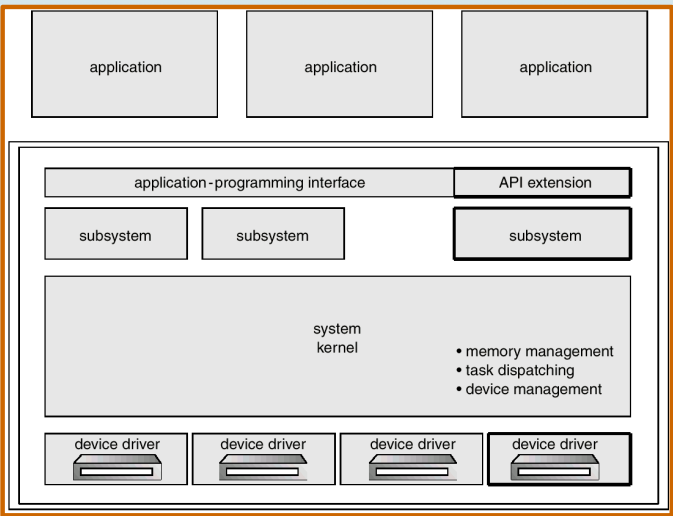
\includegraphics[width=\linewidth/2]{OS2_Layer_Structure.png}
		\caption{OS/2 Layer Structure}
	\end{figure}\par
\item 微内核(书56): OS built from many user-level processes
	\begin{itemize}
	\item 尽可能移到用户空间
	\item Communication 通过消息传递发生在用户模块间(这里会有性能损失)
	\item 便于扩展操作系统; 更易于移植操作系统到新的架构; 更可靠(更少程序运行在内核模式); 更安全
	\item Mach微内核(书56), Tru64 UNIX(书57), Mac OS X(Darwin, 部分采用Mach), QNX(书57)
	\end{itemize}
\item 模块: Core kernel with Dynamically Loadable Modules(可加载的内核模块)
	\begin{itemize}
	\item 使用面向对象的方法
	\item 每个core组件都是可分离的
	\item 每个模块通过已知接口和其他模块交互
	\item 每个模块都是在内核里可加载的.
	\item 避免每次更改都要重新编译内核
	\item 类似分层但更灵活(一个模块可以调用任何其他模块)
	\item Solaris(书58)
	\end{itemize}
\item 混合系统: Mac OS X(书58), IOS(书59), Android(书59)
\item 虚拟机: 分层结构. 视硬件和操作系统内核为硬件; 提供了和裸硬件一样的结构;
	\item 各个虚拟机相互隔离
	\item 不影响正常操作系统运行
	\item 难以实现, 因为提供准确的底层机器复制很难.
	\begin{figure}[H]
		\centering
		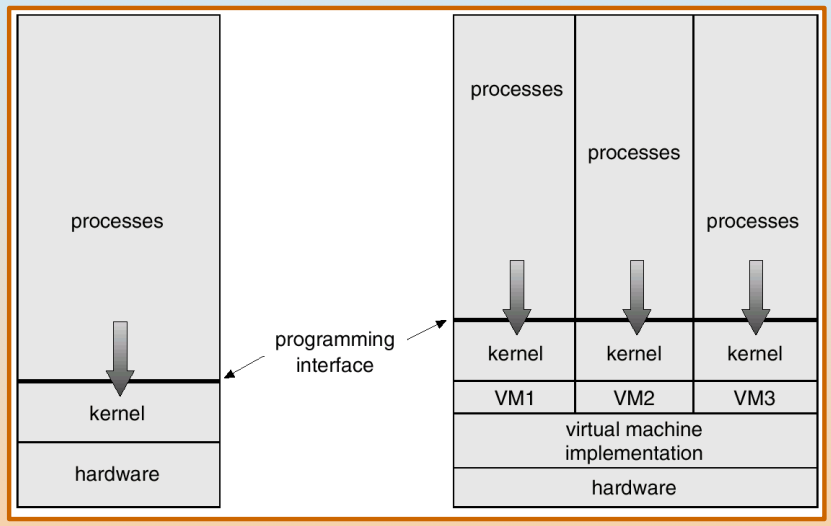
\includegraphics[width=\linewidth/2]{VM_system_models.png}
	\end{figure}\par
	\item Java 虚拟机: 运行字节码
\end{itemize}

\subsection{系统调用(书43)}
\subsubsection{程序传参方式(书45)}
\begin{itemize}
\item 用寄存器传参
\item 存参数在一个内存里的表里, 然后用寄存器传地址
\item push 到栈里
\end{itemize}

\subsubsection{系统调用类型(书46)}
\begin{itemize}
\item 程序控制
\item 文件管理
\item 设备管理
\item 信息维护
\item 通信和保护
\end{itemize}

\subsection{抽象}
\begin{itemize}
\item From transistors to 0/1 bits
\item Logic gates abstract away the details of CMOS.
\item Machine language abstracts away the details of logic gates.
\item Assembly language abstracts away the details of machine languages.
\item Programming language abstracts away the details of assembly languages
\end{itemize}

\subsection{操作系统发展历史}
\begin{itemize}
\item 1940s and 1950s: IOCS, Storage, Batch processing
\item 1960s: Time sharing, Multiprogramming; IBM OS/360, Multics
\item 1960s-1970s: UNIX(“the genius of the UNIX system is its framework, which enables
programmers to stand on the work of others”)
\item 1980s: PC; Apple, IBM, CP/M, Bill Gates; Macintosh, Windows
\item 1990s: Windows, Unix, Linux
\end{itemize}

\subsection{系统实现的问题}
\begin{itemize}
\item policy: What will be done? Mechanism: How to do it?
\item 高级语言
\item 后向兼容性
\item 算法: 线性, Tree-based, Log Structured, etc..
\item 事件模型: threads vs event loops
\item 系统生成和配置: 怎么让通用OS适应特殊的硬件
\end{itemize}

\subsection{作业调度}
\subsubsection{作业调度策略}
\begin{itemize}
\item First come first serve
\item easiest first
\item shortest time-cost first
\item earliest deadline first: 只要可行, 则按此策略必然可行.
\end{itemize}
\subsubsection{策略可行性判断}
\begin{itemize}
\item 可调度性: 存在策略使所有任务都能在截止日期前完成, 则称为可调度.
\item 可调度测试: $U=\sum\limits_{i=1}^n\frac{T_{cost}(i)}{T_{remains}(i)}$. 当U<1时可调度.(非充分必要)
\end{itemize}
\newpage
\section{进程}
进程(Linux中称任务)定义:是一个可并发执行的具有独立功能的程序关于某个数据集合的一次执行过程,也是操作系统进行资源分配和保护的基本单位.
\begin{itemize}
\item 程序的一次运行活动
\item 进程的运行活动是建立在某个数据集合之上的
\item 进程在获得资源的基础上从事自己的运行活动
\end{itemize}
\subsection{进程状态}
\begin{itemize}
\item new: 进程正在创建
\item running: 指令正在执行
\item waiting: 进程等待发生某个事件
\item ready: 进程等待分配处理器
\item terminated: 进程已经完成执行
\end{itemize}

进程控制块(PCB, 书73)
进程间切换(书74)
\subsection{基本属性}
\begin{itemize}
\item 资源的拥有者
\item 调度单位
\end{itemize}
\newpage
\section{线程}
\subsection{线程基本概念}
包括程序counter, register set, stack space; 与伙伴线程共享 代码段, 数据段, 操作系统资源. Collectively known as \textbf{job}
\begin{itemize}
\item 很适合多个线程做同样的工作, 或者多个线程之间需要共享buffer.
\item 动机(书112)
\item 优点(书113): 响应度高; 资源共享; 经济: 创建切换代价小; 多处理器体系结构的利用
\item 属性: 轻型实体; 独立调度和分派的基本单位; 可并发执行; 共享进程资源, 可伸缩性
\item 性质辨析
	\begin{itemize}
	\item 线程是进程内一个相对独立的可执行单元
	\item 线程是操作系统中的基本调度单元, 含有调度所需的必须信息
	\item 每个进程创建时, 至少需要同时为该进程创建一个线程
	\item 线程可以创建其他线程
	\item 进程是资源分配的基本单元.
	\item 由于共享资源, 线程间需要通信和同步机制
	\item 线程有生命期, 在生命期中有状态的变化
	\end{itemize}
\item 状态参数: 寄存器状态; 堆栈; 线程运行状态; 优先级; 线程专有存储器(保存线程自己的局部变量拷贝); 信号屏蔽
\item 运行状态: 执行, 就绪, 阻塞
\end{itemize}

\subsection{用户线程与内核线程}
\subsubsection{用户级线程(ULT, User Lever Thread)}
\begin{itemize}
\item 用户级线程
	\begin{enumerate}
	\item 由应用程序通过线程库完成所有线程的管理. 线程库包括线程的创建、撤消、消息和数据传递、调度执行以及上下文保护和恢复
	\item 内核不知道线程的存在
	\item 线程切换不需要核心态特权
	\item 调度是应用程序特定的
	\end{enumerate}
\item 用户级线程的内核活动:
	\begin{enumerate}
	\item 内核不知道线程, 但管理其对应进程.
	\item 线程调用系统调用时, 整个进程阻塞
	\item 线程与进程状态独立
	\end{enumerate}
\item 优缺点
	\begin{enumerate}
	\item 线程切换不需要内核
	\item 调度是应用程序特定的: 可选择最优算法
	\item 可运行在任何操作系统上(只要有线程库)
	\item 系统调用会阻塞进程上所有线程
	\item 同一进程不能有两个线程同时运行
	\end{enumerate}
\end{itemize}
\subsubsection{内核级线程(KLT, Kernel Lever Thread)}
\begin{itemize}
\item 内核级线程
	\begin{enumerate}
	\item 所有线程管理由内核完成
	\item 没有线程库, 但对内核线程工具提供API
	\item 内核维护进程和线程的上下文
	\item 线程切换需要内核
	\item 以线程为基础进行调度
	\end{enumerate}
\item 优缺点
	\begin{enumerate}
	\item 对于多处理器, 内核可以同时调度同一进程多个线程
	\item 阻塞是在线程级完成的
	\item 内核例程是多线程的
	\item 同一进程内线程切换需要内核, 速度下降
	\end{enumerate}
\end{itemize}

\subsection{进程和线程的比较}
可从调度, 并发性, 拥有资源, 系统开销来说.\\
linux所谓的线程其实是与其他进程共享资源的进程

\subsection{线程模型(书116-117)}
\begin{itemize}
\item 多对一模型: 多个用户级线程映射到一个内核线程: 一个阻塞, 全家阻塞. 无法利用多个核, 基本没人用了.
\item 一对一模型: 每个用户线程映射到一个内核线程: 更好的并发. 唯一缺点是创建一个用户线程就要对应创建一个内核线程, 开销大.(Linux, Windows)
\item 多对多模型: 多路复用多个用户级线程到同样或更少量的内核线程. 允许创建任意多用户线程, 但一个内核线程一个时刻只能调度一个, 所以并未增加并发性.
\end{itemize}
优缺点见课本

\subsection{多线程的问题}
\begin{itemize}
\item 线程取消(书127): 在线程完成之前终止进程的任务.(如并发搜索, 有一个返回了, 就都结束了)
	\begin{itemize}
	\item 异步取消: 立即终止
	\item 延迟取消: 不断检查是否应该终止. 允许让线程在安全的点取消.
	\end{itemize}
\item 线程特定数据: 同一个进程线程共享的
\end{itemize}
\newpage
\section{进程调度}
解决WHAT(分配CPU原则, 调度算法), WHEN(何时分配, 调度时机), HOW(如何分配CPU, 调度过程(进程切换))\par

控制协调进程对CPU的竞争, 即按一定的调度算法从就绪队列中选中一个进程, 把CPU的使用权交给被选中的进程.\par
\subsection{上下文切换}
\begin{itemize}
\item User process A: read(): trap to kernel mode
\item Kernel: tell disk to read sector 346761: 
	\begin{itemize}
	\item uses IVT(interrupt vector table) to handle the interrupt
	\item Disk interrupt => invoke disk driver
	\end{itemize}
\item Kernel switch to user process B
	\begin{itemize}
	\item return to user mode, but not for A
	\item A is blocked in a system call, unable to execute more instructions
	\end{itemize}
\item User process B: computes whatever it wants
\item Disk: done!
	\begin{itemize}
	\item asserts an interrupt signal
	\item CPU stops running B
	\item interrupts to kernel mode
	\item run "disk interrupt handler" code
	\end{itemize}
\item Kernel: switch to user process A
	\begin{itemize}
	\item return from interrupt, to user mode, for A, not for B
	\item B is able to execute, but not executing now. B is not running, not blocked, but ready!
	\end{itemize}
\end{itemize}

\subsection{调度算法的原则}
\begin{itemize}
\item 公平性
\item 资源利用率高
\item 交互式系统下要追求响应时间
\item 批处理系统下要追求系统吞吐量
\end{itemize}

\subsection{程序和进程的区别}
\begin{enumerate}
\item "进程"是一个动态的概念: 进程强调的是程序的一次"执行"过程,程序是一组有序指令
的集合,在多道程序设计环境下,它不涉及"执行",因此,是一个静态的概念
\item 不同的进程可以执行同一个程序: 即使多个进程执行同一个程序,只要它们运行在不同
的数据集合上,它们就是不同的进程
\item 每一个进程都有自己的生命期:当系统要完成某一项工作时,它就"创建"一个进程,程
序执行完毕,系统就"撤销"这个进程,收回它所占用的资源
\end{enumerate}

\subsection{进程特征}
\begin{itemize}
\item 进程之间具有并发性: 在一个系统中, 同时存在多个进程. 对应的多个程序同时在系统中运行, 轮流占用CPU和各种资源
\item 进程间会相互制约: 由于进程是系统中资源分配和运行调度的基本单位, 因此在对资源共享和竞争中, 必然会相互制约, 影响了各自向前推进的速度
\end{itemize}

\subsection{进程调度算法的准则(书140)}
\subsection{抢占/非抢占(书139)}
\begin{itemize}
\item 可剥夺式(可抢占式): 有更高优先级的进程就绪, 系统可以强行剥夺正在运行进程的CPU, 提供给其使用(UNIX, Linux, Windows NT/2000)
\item 不可剥夺式(不可抢占式): 某一进程调度运行后, 除非自身原因不能继续运行, 否则一直运行下去(Microsoft Windows 3.1, Apple Macintosh)
\end{itemize}

\subsection{各种调度算法(书141)}
甘特图(Gantt, 书141)可用于显示调度情况
\begin{itemize}
\item 先进先出(FIFO)/先到先服务(FCFS)(书141): 实现简单; 没考虑进程优先级
\item 短作业优先(SFJ, 最优的——平均等待时间最短): 最优但问题在于不好知道最短时间, 书143介绍了一些方法.
\item 最短剩余时间优先(SRTF, 抢占式SJF调度): 新到一个更小进程就去抢占
\item 优先级调度: 分为内部和外部优先级定义(书145); 可以是抢占/非抢占; 问题是无穷阻塞或饥饿(书145), 可用"老化"解决(动态优先数法, 与之相对的为静态优先数法)
\item 时间片轮转(Round-Robin, RR): 专为分时系统设计. 类似FCFS, 但增加抢占.
	\begin{itemize}
	\item \begin{enumerate}
		\item 每个进程获得一小段CPU时间(10-100ms)
		\item 用完后, CPU被抢占, 进程排到队尾
		\item 如果就绪队列有n个进程, 时间片为q, 那么每个进程得到1/n的时间, 每个长度不超过q时间单元.
		\item 每个进程必须等待CPU不会超过(n-1)q个时间单元
		\end{enumerate}
	\item 时间片选择: 固定/可变
	\item 与时间片大小相关的因素: 系统响应时间, 就绪程序个数, CPU能力
	\item 性能: 如果时间片很大, 则RR$\rightarrow$FIFO(FCFS); 如果时间片很短, 则响应时间短, 但上下文切换开销大
	\end{itemize}
\item 多级队列反馈调度算法: 允许进程在队列之间移动, 以实现老化; 
	\begin{itemize}
	\item 参数: 队列数量; 每个队列的调度算法; 确定升优先级/降优先级的方法; 确定需要服务时应进入哪个队列的方法
	\end{itemize}
\end{itemize}

\subsection{算法评估(书165)}
问: 如何为特定系统选择CPU调度算法?
答: 定义准则及其相对重要性, 并给出基于权重的平均值; 基于准则性能评估
\subsubsection{确定性建模(书166)}
采取用特定预先确定的系统负荷,定义在给定负荷下每个算法的性能\par
简单快速, 要求输入精确数字, 主要用于描述调度算法和提供例子\par
\subsubsection{排队模型(书167)}
系统负荷每时每刻变化, 但CPU和I/O区间的分布是确定的(通常是指数分布). 到达率和服务率$\Rightarrow$计算使用率, 平均队列长度, 平均等待时间等. \par
排队模型仅是真实系统的近似模拟\par
\subsubsection{模拟仿真(书167)}
\begin{itemize}
\item 模拟涉及对计算机系统模型进行程序设计
\item 模拟程序: 通常是事件驱动; 内部时钟
\item 随机数生成器: 根据概率分布生成进程, CPU区间时间, 到达时间, 离开时间等
\item 可采用跟踪磁带纠正驱动模拟不够精确的问题
\end{itemize}
\subsubsection{实现(书168)}
\subsection{Java线程调度简介}
JVM使用抢占式基于优先级调度的算法. 如果多线程有同优先级就用FIFIO.\par
JVM进行线程调度当: 1. 当前进程退出Runnable状态; 2. 一个更高优先级的进程进入Runnable状态.
\newpage
\section{同步}
多线程access shared data会有乱序和一致性的问题, 因此进程间必须同步\par
\begin{tabular}{|c|c|c|c|c|}
\hline
\textbf{Programs} & \multicolumn{4}{|c|}{Shared Programs} \\
\hline
\textbf{High-Level API} & Locks & Semaphores & Monitors & Send/Receive \\
\hline
\textbf{Hardware} & Load/Store & Disable Ints & Test\&Set & Comp\&Swap \\
\hline
\end{tabular}\\
\keypoint{竞争}{当两个进程竞相访问同一数据时, 就会发生竞争. 由于时间片的原因, 执行结果可能会被破坏或者被错误地解释. 为了防止竞争, 并发进程必须同步.}
\subsection{临界资源}
一次只允许一个进程使用(访问)的资源. 如: 硬件的打印机, 磁带机等; 软件的消息缓冲队列, 变量, 数组, 缓冲区等.
\begin{itemize}
\item 进程间资源访问冲突(竞争, 书176): 共享变量的修改冲突; 操作顺序冲突
\item 进程间的制约关系:
	\begin{itemize}
	\item 间接制约: 竞争, 独占分配到的部分或全部共享资源, "互斥"
	\item 直接制约: 协作, 等待来自其他进程的消息, "同步"
	\end{itemize}
\end{itemize}
\subsection{临界区(书177)}
保证当一个进程正在临界区执行时,没有另外的进程进入临界区执行. \par
临界区通用结构(书177, 图6-1)\par
\begin{itemize}
\item 临界区(critical section): 进程中访问临界资源的一段代码
\item 进入区(entry section): 进入临界区之前, 检查可否进入的一段代码. 如果可以, 设置相应"正在访问临界区"标志
\item 退出区(exit section): 用于将"正在访问临界区" 标志清除
\item 剩余区(remainder section): 代码中的其余部分
\end{itemize}
\subsubsection{解决临界区问题的原则(书177)}
\begin{itemize}
\item 互斥
\item 进步
\item 有限等待
\end{itemize}
\subsection{信号量机制}
\keypoint{信号量}{一种不需要忙等的同步工具.}
\begin{itemize}
\item 有整数型信号量, 记录型信号量, 信号集
\item 信号量s有一个整数值s.value(计数)和一个进程等待队列(s.L)
\item 只能通过初始化和两个标准的原语(wait, signal, 称为P, V操作, 书182-183)来访问(是OS核心代码, 不受进程调度打断). 初始化指定一个非负整数表示空闲资源数. 若s.value非负则表示空闲资源数, 否则表示等待临界区的进程数
\end{itemize}
\subsubsection{信号量类别}
\begin{itemize}
\item \textbf{二进制信号量}: 只允许信号量取0或1
\item \textbf{整型信号量}:PV操作(wait, signal, 书182有代码)
\item \textbf{记录型信号量}(书183有代码): 改进了整数型信号量$S\le 0$就不断忙等测试的问题, 改用让权等待, 因此需要s.L
\item \textbf{AND型信号量}: 如果单纯地交替两个mutex使用, 会造成死锁. 而AND型信号量的思想是: 一次性分配所有需要的资源, 用完后一起释放.
\begin{lstlisting}[language=c++]
Swait(S1, S2,..., Sn)
	if S1 >=1 and S2 >= 1 and ... and Sn >= 1 
		for i := 1 to n do
			Si := Si-1
		endfor
	else
		//place the process in the waiting queue associated with the first Si found with Si< 1, and set the program count of this process to the beginning of Swait operation
	endif

Ssignal(S1, S2, …, Sn)
	for i∶ = 1 to n do
		Si=Si+1;
		//Remove all the process waiting in the queue associated with Si into the ready queue.
	endfor
\end{lstlisting}
\item \textbf{信号量集}: 把AND型信号量一次一个改成一次可以多个, Swait变成Swait(S1, t1, d1,..., Sn, tn, dn)(每次要大于等于ti, 并且减di); SSignal变成signal(S1, d1, ..., Sn, dn)(每次加di)
	\begin{enumerate}
	\item Swait(S, d, d): 一个信号量, 每次要d个资源, 空闲资源少于d个就不分配.
	\item Swait(S, 1, 1): 退化为一般的记录型信号量
	\item Swait(S, 1, 0): $S\ge 0$时允许多个进程进入临界区, 但S=0时则阻止任何进程进入. 换言之, 它是个可控开关
	\end{enumerate}
\end{itemize}
\subsubsection{信号量的使用}
\begin{itemize}
\item 用信号量互斥: 设初值为1.
\begin{lstlisting}[language=c++]
semaphore mutex; //初始化为1

Process Pi:
do {
	wait(mutex);
	critical section
	signal(mutex);
	remainder section
} while(1);
\end{lstlisting}
\item 生产者-消费者问题(书185): 用记录型信号量解决(书185-186有代码); 用AND型信号量解决(生产者: Swait(empty, mutex);和Ssignal(mutex, full); 消费者: Swait(full, mutex);和Ssignal(mutex, empty);)
\item 哲学家进餐问题(书187)
\item 读者-写者问题(书186): 记录型信号量解决(书187); 用信号量集, 如下
\begin{lstlisting}[language=c++]
semaphore L(RN), mx(1); // RN is the amount of readers, mx is the lock for critical resources.

Reader:
	Swait(L, 1, 1); // Add reader if available
	Swait(mx, 1, 0); // get mx if unlocked, which means no writer
	...
	Ssignal(L, 1); // release L
	
Writer:
	Swait(mx, 1, 1; L, RN, 0); // only when mx available AND no readers are reading
	...
	Ssignal(mx, 1); // release mx for readers
\end{lstlisting}
\end{itemize}

\subsubsection{讨论}
\begin{itemize}
\item wait, signal必须成对出现. 互斥操作时它们同属一个进程; 同步操作时, 不在同个进程
\item 两个wait相邻则顺序至关重要. 两个signal相邻顺序无关紧要. 同步wait和互斥wait在一起, 同步wait总在互斥wait前.
\item 优点: 简单(可用wait, signal解决任何同步问题)
\item 缺点: 不够安全, 容易出现死锁(书184), 实现复杂
\item CAP问题: 至多同时满足两个
	\begin{itemize}
	\item Consistancy: 一致性. 所有客户端看到都是现在的数据
	\item Availability: 容许node failures
	\item Partition Tolerance: 允许network or message failures
	\end{itemize}
\end{itemize}

\subsection{管程机制}
\begin{itemize}
\item PV操作缺点: 易读性差; 不利于修改或维护; 正确性难以保证
\item 管程的引入: 把分散在各进程中的临界区集中起来管理; 防止进程有意无意的违法同步操作; 用高级语言编写易于程序正确性检验
\item 管程的属性: 共享性; 安全性; 互斥性
\item 管程组成部分: 名称; 数据结构说明; 对该数据结构操作的一组函数/过程; 初始化语句
\item 管程的形式:
\begin{lstlisting}[language=c++]
TYPE monitor_name=MONITOR;
Shared Variables Statements
define 管程内定义, 管程外可调用的函数表
use 管程外定义, 管程内将调用的函数表 
Procedure or Function
Initializations
\end{lstlisting}
\item 管程的特征:
	\begin{enumerate}
	\item 模块化: 一个管程是一个基本程序单位, 可以单独编译
	\item 抽象数据类型(ADT, 书189): 有数据还有对数据操作的代码
	\item 信息掩蔽: 管程是半透明的. 管程中的外部过程怎么实现的在外部不可见.
	\end{enumerate}
\item 管程的要素:
	\begin{enumerate}
	\item 管程中的共享变量管程外部不可见, 只能通过函数或过程间接访问
	\item 规定管程互斥进入以保证其中共享变量完整性
	\item 管程中应有进程等待队列和相应的等待与唤醒操作, 以此管理资源
	\end{enumerate}
\item 管程的条件变量: 当调用管程过程的进程无法运行时, 用于阻塞进程的一种信号量
\item 同步原语wait: 出现上述情况时, 就调用wait(condition). 等待其他进程调用signal(condition)来唤醒它.
\item 条件变量与PV操作中信号量的区别: 使用signal释放等待进程, 可能出现两个进程同时停留在管程内(signal的进程等待, 直到另一个退出; 或被释放进程等待, 直到signal的退出)
\end{itemize}

\subsubsection{管程和进程的异同}
\begin{itemize}
\item 管程是公用的数据结构, 进程是私有的数据结构
\item 管程把共享变量上的同步操作集中起来, 而临界区却分散在每个进程中
\item 管程是为了管理共享资源而建立的, 进程是为占有系统资源和实现系统并发性而引入的
\end{itemize}

\subsubsection{哲学家就餐问题的管程解决方案(书190-191)}
\subsection{Java Synchronization}
\begin{itemize}
\item synchronized, wait(), signal(): 锁机制
\item multiple notifications
\item block synchronization
\item Java semaphore: Java does not provide a semaphore, but a basic semaphore can be constructed using Java
synchronization mechanism
\item Java Monitors
\end{itemize}
\newpage
\section{进程通信(书83-)}
管道, 命名管道, 信号, 信号量, 共享内存, 内存映射, 消息队列, 套接字
\subsection{各种通信模型}
\subsubsection{管道通信}
\begin{itemize}
\item 限制: 半双工(只能单向); 只能在有亲缘关系的进程间使用
\item 管道流(s\_pipe): 可以双向传输
\item 命名管道(name\_pipe): 克服了管道没有名字, 允许任意两个进程通信
\item 为了实现管道需要: 互斥(读写互斥), 同步(写完读完就睡), 确定对方存在性.
\end{itemize}
\subsubsection{信号量通信}
信号量用来控制多个进程对共享资源的访问. 它常作为一种锁机制, 防止某进程正在访问共享资源时, 其他进程也访问该资源.
\subsubsection{消息队列通信}
\begin{itemize}
\item 是由消息组成的链表, 存放在内核中并由消息队列标识符标识
\item 消息队列克服了信号承载信息量少, 管道只能承载无格式字节流以及缓冲区大小受限等缺点.
\end{itemize}
\subsubsection{内存映射通信}
内存映射允许任何多个进程间通信,每一个使用该机制的进程通过把一个共享的文件映射到自己的进程地址空间来实现
\subsubsection{消息传递}
直接用send或receive\par
间接用信箱send(mailbox, message), recv(mailbox, message). 分为私用信箱(拥有者可读, 其他用户写); 公用信箱(操作系统创建, 核准进程可以发送读取, 在系统运行始终存在); 共享信箱(共享者有权读写). 存在一/多对一/多关系.
\subsubsection{共享存储通信}
\begin{itemize}
\item 共享内存就是映射一段能被其他进程所访问的内存, 让多个进程可以访问同一块内存空间, 这段共享内存由一个进程创建, 但多个进程都可以访问
\item 共享内存是最快的 IPC 方式(书89)
\end{itemize}
\subsubsection{Socket通信}
\begin{itemize}
\item 与其他不同的是, 可用于不同机器通信
\item 更为一般
\end{itemize}
\subsection{各种通信方式比较}
\begin{itemize}
\item 管道:速度慢,容量有限,只有父子进程能通讯
\item 命名管道(FIFO):任何进程间都能通讯,但速度慢
\item 消息队列:容量受到系统限制, 且要注意第一次读的时候, 要考虑上一次没有读完数据的问题
\item 信号量:不能传递复杂消息,只能用来同步
\item 共享内存区:容量可控,速度快,但要保持同步.
\item 有名管道虽然可以提供给任意关系的进程使用.但是由于其长期存在于系统之中,使用不当容易出错.所以普通用户一般不建议使用
\item 消息缓冲可以任意进程通信, 且使用发送接收来同步, 不用考虑其他同步问题. 但信息复制需要额外CPU时间, 不适宜信息量大的操作.
\item 共享内存改善了消息缓冲, 使得无需复制, 快, 量大. 但要同步, 且只适用于一个计算机系统内. 通过直接将共享内存缓冲区加入进程的虚拟地址实现.
\end{itemize}
\newpage
\section{死锁}
\begin{itemize}
\item 死锁的必要条件(书214): 互斥; 占有并等待; 非抢占; 循环等待
\item 系统资源分配模型(书215, 资源分配图): 如果分配图中没有环, 那么系统就没有死锁; 如果每个资源刚好只有一个实例, 那么有环就意味着死锁(书215-216)
\item 死锁发生后的处理: 
	\begin{itemize}
	\item 结束所有进程, 重启系统: 简单, 损失大
	\item 撤销死锁的所有进程
	\item 逐个撤销陷于死锁的进程
	\item 剥夺陷于死锁的进程占用的资源, 但不撤销它
	\item 根据保存的checkpoint进行回退
	\item 可能其他未死锁进程可以释放足够资源来接触死锁
	\end{itemize}
\item 死锁的预防(书217-218): 
	\begin{itemize}
	\item 破坏四个必要条件. 破坏占有并等待(执行前申请所有资源)或循环等待(没有占有资源的时候才能分配资源, 书218)比较高效.
	\item 预防措施: 静态分配(执行前前获得所有需要的资源); 层次分配策略(书218的7.4.4)
	\end{itemize}
\item 死锁的避免: 判断分配后会不会造成死锁, 会就不分配.
	\begin{itemize}
	\item 每个进程需要声明每种资源最大数目; 动态检查分配状态(取决于可用资源, 已分配资源, 进程声明的
	最大需要资源)
	\item 银行家算法. 做一个分配之前, 执行试分配, 然后用银行家算法检验安全性, 安全则分配. 需要$m*n^2$数量级的操作(书223)
	\end{itemize}
\item 死锁的检测与恢复: 允许死锁发生, 系统不断检测, 以最小代价恢复.
	\begin{enumerate}
	\item 检测时机: 当进程等待时检测死锁(系统开销大); 定时检测; 系统资源利用率下降时检测.
	\item 死锁检测算法: 每个进程和资源指定唯一编号
	\item 设置资源分配表
	\item 记录各进程与其占用资源的关系
	\item 设置进程等待表
	\item 记录各进程与要申请资源的关系
	\end{enumerate}
\item n个进程m台打印机, 打印机只能一台一台申请和释放, 每个进程需要打印机不超过m. 如果n个进程同时使用打印机的总数小于m+n, 是否会发生死锁?\\
Suppose that process $i$ needs $x_i$ printers, and has been assigned $k_i$ printers.\\
Then we get, $\sum\limits_{i=1}^{n}x_i< m+n, \sum\limits_{i=1}^{n}k_i=m$\\
Now, if deadlock occurs, $k_i< x_i, i.e., k_i+1\le x_i$\\
So, $m+n=\sum\limits_{i=1}^{n}k_i + n\le \sum\limits_{i=1}^{n}x_i<m+n$, this leads to contradiction.
\end{itemize}
\newpage
\section{内存管理}
\begin{itemize}
\item 地址变换: 将逻辑地址变换为主存中地址. 由内存管理单元(MMU)完成\\
	\begin{itemize}
	\item 什么时候确定变换关系?(书236)
		\begin{itemize}
		\item 编译时确定, 生成绝对代码: 在系统中不能移动, 否则会出错
		\item 加载时确定(静态地址变换): 实现简单, 不需要硬件支持; 但一旦加入, 要移动就比较困难, 且在程序装入的时候要将所有访问内存的地址变换.
		\item 执行时确定(动态地址变换): 这时基址寄存器称为\textbf{重定位寄存器}; 需要硬件, 但保证了灵活性. 具有给一个用户程序任意分配内存区的能力, 可以实现虚拟存储, 具有重分配能力, 对于一个用户程序可以分配到多个不同的存储区.
		\end{itemize}
	\item 动态加载(书237): 子程序调用时才加载: 更好地利用空间, 不需要操作系统特别支持, 当需要大量代码处理小概率事件时很有用
	\item 动态链接(书238)
	\end{itemize}
	
\item 主存分配: 按一定算法把某一空闲的主存区分配给作业或进程
\item 存储保护: 保证用户程序在各自的c存储区域操作, 互不干扰
	\begin{itemize}
	\item 上下界保护: 下界寄存器存放程序开始地址; 上界寄存器存放末地址(物理地址)
	\item 基址, 限长寄存器保护: 基址寄存器存放起始地址, 限长寄存器存放最大长度.(逻辑地址)
	\item 对非法访问, 上下界保护浪费CPU时间多; 对合法访问, 则一样.
	\end{itemize}
\item 虚拟存储: 使用户程序的结构大小不受主存容量容量和结构的限制.
\end{itemize}

\subsection{连续内存分配(书240)}
\begin{itemize}
\item 主存通常被分为2部分:
	\begin{itemize}
	\item 用于驻留操作系统: 为操作系统保留的部分, 通常用中断向量保存在内存低端
	\item 用于用户进程: 保存在内存高端
	\end{itemize}
\item 管理方式分类
	\begin{itemize}
	\item 单用户连续存储管理(单分区模式): 任何时刻主存只有一道程序
		\begin{itemize}
		\item 主存空间划分为系统区和用户区
		\item 地址转换: 物理地址=界限地址+逻辑地址
		\item 多采用静态重定位, 采用栅栏寄存器进行保护; 动态重定位, 采用定位寄存器进行保护;
		\item 系统利用率低
		\end{itemize}
	\item 固定分区存储管理(定长分区, 静态分区模式): 给装入的划分一块区域. 系统启动时, 操作员静态地分配.
		\begin{itemize}
		\item 静态定位方式: 地址转换时检查
		\item 动态定位方式: 专设一对地址寄存器(上下界), 硬件对相应地址进行比较
		\item 调度策略: 装入能装下它的最小分区, 可能导致分区使用不均
		\item 适合已知程序大小和频率的情况
		\item 实际系统运行时, 往往无法预知大小; 主存空间利用率仍然较低; 无法适应动态扩充主存; 分区数目预先确定, 限制了多道程序的数量
		\end{itemize}
	\item 可变分区存储管理(变长分区模式, 书241)
		\begin{itemize}
		\item 数据结构由已分配区表和未分配区表构成
		\item 分配算法(书241-242): 首次适应; 最佳适应; 最坏适应; 下次适应; 快速适应
		\item 存储速度和资源利用率上, 首次适应和最佳适应要比最差适应好; 而首次适应要快些.
		\item 回收时考察相邻分区能否合并
		\end{itemize}
	\end{itemize}
\item 动态定位/静态定位
\end{itemize}
\subsubsection{连续内存分配的问题}
\begin{itemize}
\item 碎片(书242): 首次适应和最优适应都有外部碎片(解决方法: 紧缩. 移动内存, 将空闲的整合为一块(只有动态重定位可以); 允许逻辑空间不连续(分段和分页)). 而按固定大小的块分配时, 会有内部碎片
\end{itemize}
\subsection{分页}
\begin{itemize}
\item 解决了进程增长, 碎片化, 交换长延迟的问题
\item 动态重定位
\item 可以做到0外部碎片, 平均$\frac{1}{2}$page per region的内部碎片
\item 新问题
	\begin{itemize}
	\item 两次访存. 一次取页号, 一次取数据
	\item 页表规模过大. 采用多级页表, 避免连续分配过大空间.(但总页表空间会变大, 比如还要加上页表的表的空间)
	\end{itemize}
\item 实现: 页表基址寄存器指向页表(PTBR, 书248), 页表限长寄存器(PTLR, 用于避免所有页都建立条目的开销)表明页表长度; 相联存储器解决二次访存问题(书248)
\item 基于TLB的有效访问时间: EAT(Effective Access Time)=$(t+\epsilon)\alpha+(2t+\epsilon)(1-\alpha)$, $\alpha$为命中率(在TLB中找到的概率), t为访存一次需要时间, $\epsilon$为TLB查找需要时间.
\item 存储保护: 可以提供只读只写只执行保护. 还可以提供有效-无效位
\item 共享页: 这是分页的优点之一——可以共享代码(如文本编辑器代码等可重入代码或纯代码, 书251). 每个进程保留私有代码和数据
\end{itemize}
\subsection{分段(书242-244)}
一个程序是一些段的集合, 一个段是一个逻辑单位, 如: 主函数, 函数过程方法对象, 局部变量全局变量, 堆栈, 符号表, 数组.
\begin{itemize}
\item 段表: 将<段号, 偏移>这样的二维地址映射到一维物理地址.
\item 段基地址, 段界限: 段表的条目内容
\item 段共享: 通过不同作业段表中的项指向同一个段基址来实现
\end{itemize}
\subsection{分段和分页的主要区别}
\begin{itemize}
\item 页是信息的物理单位, 分页是由于系统管理需要, 减少外部碎片, 提高内存利用率. 段则是信息的逻辑单位, 它含有一组意义相对完整的信息, 是为了更好地满足用户需要.
\item 页大小固定且由系统决定, 系统把逻辑地址划分为页号和页内地址, 是硬件实现的. 段长不固定, 取决于用户程序, 通常是编译的时候根据信息性质划分的.
\item 分页的作业地址空间是唯一的, 即单一的线性地址空间; 分段的作业则是二维的程序员.
\end{itemize}
\newpage
\section{虚拟内存}
\subsection{背景(书264)}
\begin{itemize}
\item 事实:
	\begin{itemize}
	\item 数组, 链表和表通常分配了比实际所需要更多的内存
	\item 程序的某些特点很少使用, 即使要完整程序, 也并非同时.
	\item 时空局部性
	\end{itemize}
\item 优点(书265)
	\begin{itemize}
	\item 逻辑地址空间能比物理地址空间大: 保存部分程序在内存中, 可运行一个比物理内存要大的程序
	\item 可以有更多程序同时运行
	\item 允许若干个进程共享地址空间
	\item 进程创建更高效(共享页面, 书265)
	\end{itemize}
\item 实现: 请求分页式管理, 请求分段式管理, 请求段页式管理
\end{itemize}

\subsection{请求调页(书266)}
\begin{itemize}
\item 仅在需要时才加载页面(甚至不是加载整个进程): I/O小, 需内存小, 响应快, 适合多用户
\item 驻留标志: 以表示页是否在主存里. 缺页错误处理流程(书267)
\item 硬件支撑(MMU): 完成逻辑地址到物理地址的转换, 并产生相应中断(缺页终端, 越界中断), 主要由页表基址寄存器和快表TLB组成.
\begin{figure}[H]
	\centering
	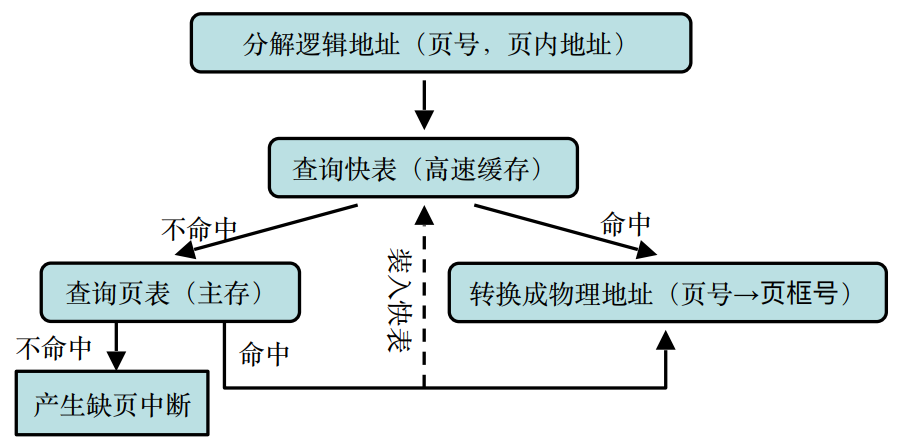
\includegraphics[scale=0.3]{MMU.png}
	\caption{MMU工作流程}
\end{figure}\par
\item 没有空闲帧可以放时, 就要Swapping.
\end{itemize}

\subsection{请求分页式存储管理}
\begin{itemize}
\item 何时装入: 请页式调入(缺页中断驱动, 一次一页); 预调式调入(按算法动态预测调入若干页)
\item 消除策略: 请页式清除(仅当一页被选中替换时, 该页若已修改则写回辅存); 预约式清除(成批写回, 通常在替换前).
\end{itemize}

\subsection{请求分页性能}
有效访问时间=$(1-p)\times ma+p\times $缺页错误时间. (ma是内存访问时间, p是缺页错误概率(页面替换算法, 主存页框数, 页面大小, 程序特性), 缺页错误时间=页错误开销+换出开销+换入开销+重启开销)\par
用COW(copy on write)技术提高fork的性能.\par

\subsubsection{帧分配算法(书282)}
\begin{itemize}
\item 固定分配: 在一个进程的生命周期中, 分配给它固定帧数. 有平均分配, 按比例分配, 优先权分配
\item 可变分配: 缺页次数多的进程分配更多帧
\item 全局分配与局部分配(书282)
\end{itemize}
\subsubsection{页替换算法(书275)}
\begin{itemize}
\item FIFO: 性能一般. 有Belady异常(增加帧数但缺页率反而增高, 书276)
\item 最优页替换(OPT算法): 用于比较研究. 没有Belady异常
\item 随机替换: 
\item 最近最少使用算法(LRU): 没有Belady异常
	\begin{itemize}
	\item 计数器实现: 每次引用就保存时间域(书277). 还要考虑时钟溢出, 页表更改时也要保留好时间.
	\item 栈(双链表)实现: 被引用就移到栈顶. 无需查找. 最坏情况要改6个指针.
	\end{itemize}
\item 近似LRU算法: 引用位. 每个页与一页关联, 引用了就置1. 缺点是时间顺序未知. 可以改进:
	\begin{itemize}
	\item 额外引用位算法(书278): 用8位存排序信息, 定时地将引用位移到最高位, 其他位右移.
	\item 第二次机会算法(时钟算法是一种实现方法, 书278): 
	\item 增强型第二次机会算法(书279): 用引用位和修改位
	\end{itemize}
\item 最不常使用(LFU, 书279): 如果一个页面大量使用后再也不使用就会有问题. 可以考虑定期计数器右移.
\item 最经常使用(MFU): 和LFU两个基于计数的算法都实现昂贵.

\end{itemize}

\subsection{内存抖动}
如果一个进程没有足够页, 那么缺页概率会很高, 这将导致CPU利用率低下及操作系统认为需要增加多道程序数
\subsubsection{策略}
\begin{itemize}
\item 局部置换算法: 如果一个进程开始抖动, 就采用局部置换, 这样就不能从另一个进程获得帧, 从而避免影响另一个进程. 但缺页错误平均等待时间也会增加.
\item 优先级置换算法
\item 缺页率高就多分配些, 低就收回些
\item 提供足够的帧: 问题是怎么知道需要多少? 局部性模型, 工作集模型.(书285)
170页
\item 改变页大小
	\begin{itemize}
	\item 减小页大小$\rightarrow$增加页表大小:
		\begin{itemize}
		\item 碎片: 小页更好利用内存
		\item I/O开销: 寻道和延迟时间远大于传输时间, 需要小页
		\item 局部: 较小页允许每个页更精确的匹配程序局部
		\end{itemize}
	\item 增加页大小: 碎片增加
	\item 提供多种页大小
	\end{itemize}
\end{itemize}

\subsection{内存模型}
缓存一致性(Cache Coherence)和内存一致性(Memory Consistency, 更像是连贯性)

\newpage
\section{大容量存储结构}
\begin{itemize}
\item 介质种类: 磁盘(书367), 磁带(数368), 光盘
\item 物理块: 文件系统中, 存储设备被划分为大小相等的物理块, 文件信息也划分成逻辑块, 以块为单位进行存储传输和分配.
\item RAM存储: 硬盘便宜, DRAM快得多
\item 固态硬盘(书368): 包括 带电池的DRAM, 闪存技术等
\item 总线: 一般有CPU-Memory总线和I/O总线
	\begin{itemize}
	\item PCI: 快而相对短, 可直接连接快速设备, 也可以连接长而慢的I/O总线
	\end{itemize}
\end{itemize}
\subsection{磁盘}
\begin{itemize}
\item 物理地址: $<$设备号, 磁头号(盘面号), 磁道号(柱面号), 扇区号$>$
\item 访盘的三个动作(书367): 寻道, 旋转延迟, 数据传输
\item 固定头磁盘: 每个磁道一个磁头, 速度快成本高; 移动头磁盘: 每个盘面一个磁头, 速度慢成本低
\item 度量指标: 
	\begin{itemize}
	\item Response Time(响应时间)=Queue(排队等待处理时间) + Disk Service Time
	\item 吞吐量(Throughput)
	\item Disk Latency
		\begin{align*}
		Disk\ Latency &= Queueing\ Time + Controller\ Time \\
		&+ Seek\ Time\ \mbox{(8ms-12ms)} \\
		&+ Rotation\ Time\ \mbox{(16ms-8ms per revolution, i.e., 8ms-4ms average latency)} \\
		&+ Transfer\ Time\ \mbox{usually 512B-1KB per sector, 2-50MB per second}
		\end{align*}
	\end{itemize}
\item 通过数据冗余提高访问速度
\item Disks vs Memory\\
	\begin{tabular}{|c|c|c|}
	\hline
	 & Disks & Memory \\
	\hline
	Smallest write & sector & bytes \\
	\hline
	Atomic write & sector & byte, word \\
	\hline
	Random Access & 5ms & 50ns \\
	\hline
	Sequential Access & 200MB/s & 200-1000MB/s \\
	\hline
	Cost & \$.002MB & \$.10MB \\
	\hline
	Crash & non-volatile & volatile \\
	\hline
	\end{tabular}
\end{itemize}

\subsubsection{Dependability, Reliability and Availability}
\begin{itemize}
\item Dependability:
	\begin{itemize}
	\item Faliure: actual deviates from specified behavior
	\item Error: defect that results in failure
	\item Faults: cause of error
		\begin{itemize}
		\item Hardware Faults: fail to perform as design
		\item Design Faults: faults in software or in HW
		\item Operation Faults: Oprator and user mistakes
		\item Environmental Faults: Fire, power failure, etc.
		\end{itemize}
	\end{itemize}
\item Reliablity:用Mean Time to Failure(MTTF)衡量
	\begin{itemize}
	\item Fault Avoidance
	\item Fault Tolerance
	\item Error Removal
	\item Error Forecasting
	\end{itemize}
\item Availability: 用MTTF/(MTTF+MTTR)衡量, 其中MTTR是Mean Time to Repaire
\end{itemize}

\subsubsection{磁盘(移动臂)调度算法(书371)}
\begin{itemize}
\item 先到先服务(FCFS)
\item 最短寻道使劲按优先(SSTF): 选择最接近磁头位置的待处理请求.
\item 扫描算法(SCAN, 又称电梯算法): 从磁盘一端开始向另一端移动, 到另一端时, 移动方向反转, 继续处理.
\item C-SCAN: 移动到磁盘另一端后, 立即返回开头, 中间不做任何处理, 以提供更均匀的等待时间.
\item LOOK/C-LOOK调度: SCAN/C-SCAN的改进. 只移动到最远的请求为止.
\end{itemize}
\subsubsection{算法评价}
\begin{itemize}
\item 比较合理的默认算法: SSTF和LOOK
\item FCFS和SCAN算法单位时间内处理I/O请求多(吞吐量大), 但请求的等待时间可能较长
\item SCAN算法适宜磁盘负载重的系统, 要扫过所有柱面, 性能不够好
\item 分步扫描算法使得I/O请求等待时间之间差距最小, 吞吐量适中
\item 电梯调度算法杜绝饥饿, 性能适中
\item 循环扫描算法适应不断有大批量柱面均匀分布的I/O请求, 且磁道上存放记录数量较大的情况
\end{itemize}
\subsubsection{磁盘存储性能}
\begin{itemize}
\item 速度和可靠性是主要瓶颈, 文件系统应尽量减少磁盘访问次数
\item 块高速缓存: 系统在内存中保存一些块作为缓存
\item 合理分配磁盘空间: 把可能顺序存取的块放在一起, 最好在同一柱面上
\item 磁盘调度: 旨在降低平均磁盘服务时间, 达到公平高效.
\end{itemize}

\subsection{RAID独立磁盘冗余阵列(书378)}
用一组较小容量的、独立的、可并行工作的磁盘驱动器组成阵列来代替单一的大容量磁盘,并加入冗余技术,数据能够以多种方式组织和分布存储\par
数据分布存储, 提高了单个I/O请求的处理性能; 数据的冗余, 提高了系统的可靠性

\subsection{驱动调度技术}
\begin{itemize}
\item 系统运行时,同时会有多个访问辅助存储器的进程请求输入/输出操作,操作系统必须采一种种调度策略,使其能按最佳的次序执行各访问请求
\item 若干个输入输出请求服务所需的总时间越少, 则系统效率越高
\item 影响存取速度的因素:
	\begin{itemize}
	\item 调度算法
	\item 信息在辅存上的排列方式
	\item 存储空间的分配方式
	\end{itemize}
\item 提高磁盘I/O的方法: 提前读, 延迟写, 虚拟盘
\end{itemize}

\subsection{用户对外存的要求}
\begin{itemize}
\item 读写不涉及硬件细节, 使用逻辑地址和逻辑操作
\item 存取速度尽可能快, 容量大且空间利用率高
\item 存放信息安全可靠
\item 可以方便地共享, 动态扩缩, 携带拆卸
\item 代价尽可能小
\end{itemize}

\newpage
\section{文件系统}
管理文件的软件即存取和管理信息的机构. 用统一的方式管理用户和系统信息的存储, 检索, 更新, 共享和保护, 并为用户提供一整套方便有效的文件使用和操作方法. 它是管理文件所需要的数据结构(目录, 索引表等)的总体.\par
用户看来: 文件系统呈现在用户面前的是一个文件由什么组成, 如何命名, 如何保护文件, 可以进行何种操作等等.\par
操作系统需要考虑: 文件目录怎样实现, 怎么样管理存储空间, 文件存储位置, 磁盘实际运作方式(与设备管理的接口)等.\par
\begin{itemize}
\item 文件系统面向用户的功能
	\begin{itemize}
	\item 文件的按名存取
	\item 文件目录建立和维护
	\item 实现逻辑文件到物理文件的转换
	\item 文件存储空间的分配和管理
	\item 提供合适的文件存取方法
	\item 实现文件的共享, 保护和保密
	\item 提供一组可供用户使用的文件操作
	\end{itemize}
\item 文件系统的特点
	\begin{itemize}
	\item 友好的用户接口. 用户只要对文件操作, 不用管结构和存放位置
	\item 对文件按名存取, 对用户透明
	\item 某些文件可以被多个用户或进程共享
	\item 可存储大量信息
	\end{itemize}
\item 文件操作(书311): 创建, 改写, 读取, 重定位文件, 删除, 截短, 重命名, 拷贝, 扩展
\item 文件分类: 对不同文件进行管理, 提高系统效率, 提高用户界面友好性
	\begin{itemize}
	\item 按文件性质和用途分类: 系统文件, 用户文件, 库文件
	\item 按信息保存期限分类: 临时文件, 永久文件, 档案文件
	\item 按保护方式分类: 只读, 读写, 可执行, 不保护
	\item 按文件的逻辑结构分类: 流式文件, 记录式文件
	\item 按物理结构: 连续文件, 链接文件, 索引文件
	\item 按存取方式: 顺序存取, 随机存取
	\item 按设备类型: 磁盘, 磁带, 打印
	\item 按文件内容: 普通文件, 目录文件, 特殊文件(字符设备文件, 网络设备文件等)
	\end{itemize}
\item 文件类型(书315)
\item 文件属性: 用于文件的管理控制和安全保护
	\begin{itemize}
	\item 基本属性: 文件名, 所有者, 授权者, 长度等
	\item 类型属性: 普通文件, 目录文件, 系统文件, 隐式文件, 设备文件等
	\item 保护属性: 读, 写, 可执行, 可更新, 可删除, 可改变保护, 归档
	\item 管理属性: 创建时间, 最后存取时间, 最后修改时间等
	\item 文件保护属性: 防止文件被破坏. 定时转储, 多副本; 建立用户三元组(用户, 对象, 存取权限)防止用户有意无意非法操作造成问题
	\end{itemize}
\item 与文件组织和存储相关概念
	\begin{itemize}
	\item 卷: 是物理存储介质的单位. 物理卷和物理设备不总是一致
	\item 块: 存储介质上连续信息组成的一个区域, 也叫物理记录
	\item 逻辑记录: 按信息在逻辑上划分的信息单位, 是应用程序处理的单位
	\item 存储记录: 指附加了操作系统控制信息的逻辑记录, 是文件管理程序的处理单位
	\item 逻辑记录可以对应多个块, 一个块可以对应多个逻辑记录. 书和章节相当于文件和逻辑记录, 是逻辑概念; 而册和页相当于卷和块, 是物理概念.
	\end{itemize}
\end{itemize}

\subsection{文件结构}
\begin{itemize}
\item 文件的逻辑结构
	\begin{itemize}
	\item 无结构文件: 又称流式文件. 基本信息单位是字节或字. 如大量源程序, 可执行文件, 库函数等. 无格式限制
	\item 有结构文件: 有格式限制. 如一张表. 简单的结构有行, 定长记录, 变长记录; 复杂的有格式化的文档, 可重定位文件.
	\item 选择逻辑结构应遵循:
		\begin{itemize}
		\item 当用户对文件信息进行修改操作时, 给定的逻辑结构能尽可能减少对已存储好的文件信息的变动
		\item 需要时应能够尽可能快地查找到记录或基本信息单位
		\item 尽量使占据空间小
		\item 便于用户操作
		\end{itemize}
	\end{itemize}
\item 文件的物理结构
	\begin{itemize}
	\item 顺序文件(书317), 连续文件: 存取效率最高; 但创建时需要指出文件大小, 查改性能差.
	\item 链接文件: 使用链接字或指针表示记录间的串联关系. 存储空间利用率高, 顺序存取效率高; 随机存取效率低(访问最后的内容相当于要访问整个文件)
	\item 直接文件: 在记录的关键字和物理地址之间建立某种映射(如哈希散列). 问题在于哈希冲突等.
	\item 索引文件(书318): 为每个文件建立一张索引表, 每个表目包含一个记录键及对应存储位置. 优点: 保持了链接结构的优点, 但又能随机存取, 满足了动态增长, 插入删除的要求, 充分利用了外村空间; 缺点: 寻道次数多和寻道时间长, 索引表本身带来了系统开销. 索引的三种结构: 直接地址结构, 索引结构, 计算寻址结构.
	\end{itemize}
\end{itemize}
\subsection{存取访问方法(书317)}
顺序存取, 直接存取, 索引存取
\subsection{文件目录}
\subsubsection{文件控制块(FCB)}
\begin{itemize}
\item 文件控制块(FCB): 每个文件目录项对应一个文件的信息描述, 该目录项又称为文件控制块(FCB). 找到了一个文件的FCB, 就得到了文件的有关信息, 就能够对它进行所需要的操作了.
	\begin{itemize}
	\item 文件存取控制信息: 文件名, 用户名, 文件主存取权限等
	\item 文件结构信息: 文件逻辑结构, 文件物理结构
	\item 文件使用信息: 已打开该文件的进程数, 文件的修改情况等
	\item 文件管理信息: 文件建立日期, 文件访问日期等
	\end{itemize}
\item UNIX的"inode"
\end{itemize}
\subsubsection{文件目录结构(书320)}
\begin{itemize}
\item 一级目录结构: 线性表
	\begin{itemize}
	\item 优点: 简单, 易实现
	\item 缺点: 重名问题, 难以实现文件共享, 文件平均检索时间长
	\end{itemize}
\item 二级目录结构: 第一级管理用户; 第二级管理用户下文件
	\begin{itemize}
	\item 优点: 解决了重名和文件共享问题, 用户名和文件名查找时间低
	\item 缺点: 增加了系统开销
	\end{itemize}
\item 
	\begin{itemize}
	\item 优点
		\begin{itemize}
		\item 较好反映数据之间层次关系
		\item 不同文件可以重名, 只要不在一个目录内
		\item 容易以目录为单位进行文件保护, 保密和共享
		\end{itemize}
	\item 缺点
		\begin{itemize}
		\item 按路径逐层检查, 多次访盘影响速度
		\end{itemize}
	\end{itemize}
\end{itemize}

\subsection{文件系统的挂载和使用}
\begin{itemize}
\item Windows/Dos系统中, 不需要用户显式进行文件卷挂载操作
\item UNIX/Linux系统中, 每个卷需要安装才能使用. 文件系统分为基本文件系统和可装卸的子文件系统两部分(mount操作, 如mount /dev/hda5 /mnt/diskD)
\end{itemize}
\subsection{文件共享(书327)}
\begin{itemize}
\item 文件共享: 不同用户(进程)间共用一个文件
\item 三种形式:
	\begin{itemize}
	\item 被多个用户使用, 有存取权限控制
	\item 被多个程序使用, 各用自己的读写指针
	\item 被多个程序使用, 但共享读写指针
	\end{itemize}
\item 可以节省大量外存空间, 有效减少文件复制而增加的访问外存次数, 进程间可以通过文件交换信息
\item UNIX中文件共享方式: 静态共享, 动态共享, 符号链接共享
	\begin{itemize}
	\item 静态共享: link/unlink. 构建新目录项, 并对inode连接计数i\_nlink加1. 链接实际上是共享已存在文件的索引节点inode. 只有当i\_nlink减为0, 文件才被真正删除
	\item 动态共享: 是系统中不同用户进程并发访问的情况. fork后, 两个进程的打开文件表是一样的(被复制的), 从而达到共享同一位移指针的目的. 而如果多用户共享, 希望独立读写, 则应分别设置读写位移指针.
	\end{itemize}
\end{itemize}

\subsection{虚拟文件系统}
\subsubsection{虚拟文件系统的目标}
\begin{itemize}
\item 同时支持多种文件系统
\item 系统中可安装多个文件系统
\item 为用户提供一致的接口
\item 提供网络共享文件支持
\item 可扩充新的文件系统
\end{itemize}
\subsubsection{虚拟文件系统基本思路}
\begin{itemize}
\item 对多个文件系统的共同特征抽象, 形成一个与具体文件系统无关的虚拟层, 并在此层上定义对用户的一致性接口.
\item 文件系统具体实现使用类似开关表技术进行文件系统的转接, 每个文件系统是自包含的, 实现各文件系统的具体细节.
\end{itemize}

\subsection{文件系统的保护(书331)}
\begin{itemize}
\item 文件系统的可靠性
	\begin{itemize}
	\item 坏块问题
	\item 备份: 转储形成多个副本. RAID; 海量转储(定期拷贝到后援存储器); 增量转储(只转出修改过的文件)
	\item 恢复
	\item 文件系统的一致性: 若写回之前系统崩溃, 则文件系统会不一致, 需要在系统重启时, 检查磁盘块和目录系统
	\item 一致性检查工作过程: 一张表记录每块在文件中出现次数, 一张表记录每块在空闲块表中出现次数. 空闲和非空闲应互补. 否则可能有重复块或块丢失
	\end{itemize}
\item 文件系统的安全性
	\begin{itemize}
	\item 数据丢失, 灾难等: 通过备份解决
	\item 积极或消极的入侵者
	\item 安全性设计原则
		\begin{itemize}
		\item 系统设计必须公开
		\item 缺省属性应该不可访问
		\item 检查当前权限
		\item 给每个进程赋予最小可能权限
		\item 保护机制应简单一致, 嵌入到系统底层
		\item 采取的方案必须可接受
		\end{itemize}
	\end{itemize}
\end{itemize}
\subsubsection{文件保护机制}
\begin{itemize}
\item 文件保护
\item 用户验证: 检验身份
\item 存取控制: 一级(识别访问者, 文件主, 文件主的同组用户, 其他用户); 二级(操作权限分类, 读写执行等)
\end{itemize}
\subsection{文件系统的实现}
\subsubsection{文件系统类型}
\begin{itemize}
\item FAT文件系统(MS-DOS文件系统)
\item FAT32(vfat): 在FAT基础上增加了对长文件名(最多256B)的支持
\item NTFS: Windows NT使用的. 有很强的安全特性和文件系统恢复功能, 可以处理巨大的存储媒体, 支持多种文件系统
\item S51K/S52K(sysv): AT\&T UNIX S V操作系统使用的1KB/2KB文件系统
\item ext2(二级扩展文件系统): 是Linux使用的高性能磁盘文件系统, 是对Minux的ext的扩展. 支持256B文件名, 最大支持4TB文件系统大小
\item HPFS(高性能文件系统): OS/2操作系统使用的
\item CD-ROM文件系统(iso9660): 符合iso9660标准支持的CD-ROM文件系统
\item UDF通用磁盘格式文件系统
\end{itemize}
\subsubsection{目录实现}
\begin{itemize}
\item 线性列表
\item 哈希表
\end{itemize}
\subsubsection{文件存储空间管理}
\begin{itemize}
\item 位示图, 空闲为0, 已分配为1
\item 空闲区表: 表中每个条目记录磁盘空间中一个连续空闲盘区信息.(起始块号, 连续块数, 状态)
\item 空闲块链: 空闲块形成一个链表, 也称空白串联文件
\item 成组链接: 根据磁盘块数开辟若干专门用来登记系统当前拥有空闲块的块号. (UNIX)
\item 内存中需要表目: 系统打开文件表, 用户打开文件表(每个进程一个在PCB中)
\end{itemize}
\subsection{文件系统效率和性能}
\begin{itemize}
\item 取决于: 磁盘分配和目录管理算法; 保留在文件目录条目中的数据类型
\item 性能:
	\begin{itemize}
	\item 磁盘缓存: 一块独立内存, 装载常用块
	\item 优化顺序访问的技术: 马上释放(free-behind)和预先读取(read-ahead)
	\item 留出一块内存作为虚拟磁盘
	\end{itemize}
\end{itemize}

\subsection{基于日志结构的文件系统}
每次更新记录为一个transaction, 一旦写入就认为是committed, 当transaction完成就从日志中删除, 如果系统崩溃, 在日志中保存的transaction仍必须执行.

\newpage
\section{设备管理}
\begin{itemize}
\item 计算机的外围设备分为: 存储型设备, 输入输出型设备
\item 设备管理的目的: 方便用户使用各种各样的外围设备, 同时提高各种外围设备的并行性, 从而提高其利用率
\item 目标和功能
	\begin{itemize}
	\item 根据用户请求, 控制各类设备实现用户的目标
	\item 向用户提供方便的设备接口, 屏蔽底层硬件细节区别
	\item 利用各种技术(中断, DMA, 通道, 缓冲), 提高设备运行效率
	\item 实现对设备的管理和保护
	\end{itemize}
\item 基本内容: 外围设备中断处理, 缓冲区处理, 外围设备登记和使用情况跟踪以及分配和去配
\item 外围设备驱动调度, 虚拟设备及其实现
\end{itemize}

\subsection{设备分类}
\begin{itemize}
\item 按传输速率: 低速(B-百B/s, 键鼠语音), 中速(KB-10KB/s, 行式打印机, 激光打印机等), 高速(100KB-MB/s, 磁带机, 光盘机)
\item 按信息交换的单位: 块设备(Block Device, 磁盘等, 传输速率较高, 可寻址, DMA), 字符设备(Character Device, 一般用于输入输出, 传输速率较低, 不可寻址, 中断)
\item 按资源分配: 独占设备(终端, 打印机), 共享设备(磁盘), 虚拟设备(将一台独占设备变换为多个用户共享的逻辑设备)
\item 按输入/输出
\item 按存取方式: 顺序/随机
\end{itemize}

\subsection{I/O控制方式}
\begin{itemize}
\item 按功能强弱及与CPU并行度: 轮询$<$中断$<$DMA$<$通道
	\begin{itemize}
	\item 询问: 不断查询, CPU和设备串行, 效率低
	\item 中断: 数据传输时仍需要CPU, 仍为串行, 效率有所提高.
	\item DMA: I/O设备可以直接和主存交换数据, DMA设备与CPU共享对总线的控制, 可并行工作. 缺点是CPU还需要在块与块之间对I/O操作进行干预.
	\item 通道: 只在开始的时候执行相应指令, 结束时中断通知代码处理. 完全并行, 效率高. 瓶颈在于通道相对设备较少, 会造成数据交换阻塞.
		\begin{itemize}
		\item 字节多路通道: 按字节交叉方式工作. 每个通道完成一个字节交换后便让出通道
		\item 数组选择通道: 字节多路通道不适于高速设备. 这种方式在一定时间只能执行一个通道的程序, 且独占, 直至完成释放.
		\item 数组多路通道: 将二者结合
		\end{itemize}
	\end{itemize}
\end{itemize}


\subsection{总线系统}
PC/XT$\rightarrow$ISA$\rightarrow$MCA$\rightarrow$EISA$\rightarrow$VESA$\rightarrow$PCI$\rightarrow$USB$\rightarrow$SCSI
\begin{itemize}
\item ISA(Industry Standard Architecture): 原先带宽8位, 2Mb/s; 后为16位, 16Mb/s
\item EISA(Extended ISA): 32位, 32Mb/s
\item 局部总线: 将多媒体卡, 高速LAN卡, 高性能显卡等从总线分离, 直接接到CPU总线上
\item VESA(Video Electronic Standard Association): 32位, 132Mb/s, 控制器无缓冲, 甚至不支持奔腾
\item PCI(Peripheral(外围的) Component Interface): 支持64位系统, 在CPU和外设之间加了一层复杂的管理系统, 用于协调数据传输和提供一致的接口. 能适应高频率的CPU
\item USB技术(通用串行总线): 突破了接口标准不一致和有限接口数量两个局限. 以WDM(Windows Driver Model, 包含一套通用I/O服务和二进制兼容的设备驱动程序)模型为基础. 支持同步数据传输方式和异步数据传输方式, 低速1.5Mbps-全速12Mbps乃至上百Mbps. 可以主动为外部设备提供电源, 允许热插拔. \textbf{控制器}主要负责执行由控制器驱动程序发出的命令. \textbf{控制器驱动程序}在控制器和USB设备之间建立通信信道. \textbf{USB芯片驱动程序}提供了对USB的支持. 有等时传输方式(固定传输速率不断传输), 中断传输方式(传输小但需及时处理的数据), 控制传输方式(处理主机的数据传输命令), 批量传输方式(用来传输要求正确无误的数据, 打印机等)
\item SCSI(Small Computer System Interface): 可将新型告诉I/O设备增加到计算机中, 智能化控制降低了计算机系统的负担
\end{itemize}

\subsection{缓冲技术}
\begin{itemize}
\item 动因
	\begin{itemize}
	\item 改善CPU与外围设备速度不匹配的矛盾
	\item 协调逻辑记录和物理记录大小不一致的问题
	\item 减少I/O操作对CPU执行的中断次数
	\item 放宽CPU对中断响应时间的要求
	\end{itemize}
\item 分类: 单缓冲, 双缓冲(两个缓冲区轮流工作), 多缓冲(多级缓冲组成循环缓冲)
\end{itemize}

\subsection{高速缓存}
\begin{itemize}
\item 保留数据拷贝的高速缓存: 总是数据的拷贝, 性能的关键
\item 缓冲与高速缓存: 缓冲只是保留数据仅有的一个现存拷贝; 高速缓存提供了一个驻留在其他地方的数据的一个高速拷贝
\end{itemize}

\subsection{即插即用技术(Plug and Play, PnP)}
自动识别, 配置...

\subsection{调度}
\begin{itemize}
\item 操作系统为每一个设备维护一个请求队列来实现调度.
\item 独立性: 作业与物理设备独立, 作业指定逻辑设备而非物理设备
\item 设备分配: FCFS, 优先级算法
\end{itemize}

\subsection{虚拟设备}
\begin{itemize}
\item 作用: 使独立使用的设备变成可共享设备; 处理器与外围设备速度匹配.
\item 假脱机: 比如打印机一次只能服务一个请求, 就先假脱机到一个独立的磁盘文件上.
\item 设备预约: 提供对设备的独占访问. 小心死锁.
\end{itemize}

\subsection{错误处理}
\begin{itemize}
\item 预防, 恢复磁盘读
\item 返回调用状态信息
\item 系统日志记录出错报告
\end{itemize}






\end{document}
